\chapter{Artificial Intelligence}
\setcounter{secnumdepth}{5}
\label{ch:AI}
\setlength\lineskip{0pt}
\vspace*{15pt}

\definecolor{codegreen}{rgb}{0,0.6,0}
\definecolor{codegray}{rgb}{0.5,0.5,0.5}
\definecolor{codepurple}{rgb}{0.58,0,0.82}
\definecolor{backcolour}{rgb}{0.95,0.95,0.92}
\definecolor{deepred}{rgb}{0.6,0,0}
 
\lstdefinestyle{mystyle}{
    backgroundcolor=\color{backcolour},   
    commentstyle=\color{codegreen},
    keywordstyle=\color{blue},
    numberstyle=\tiny\color{codegray},
    stringstyle=\color{codepurple},
    basicstyle=\footnotesize,
    breakatwhitespace=false,         
    breaklines=true,                 
    captionpos=b,                    
    keepspaces=true,                 
    numbers=left,                    
    numbersep=5pt,                  
    showspaces=false,                
    showstringspaces=false,
    showtabs=false,                  
    tabsize=2
}
 
\lstset{style=mystyle}

Two of the main techniques used in order to try to discover causal relationships are Graphical Methods (such as Knowledge Graphs and Bayesian Belief Networks) and Explainable AI. These two methods form in fact the basis of the Association level in the Causality Hierarchy (Figure \ref{pyr}), enabling us to answer questions such as: What different properties compose an entity and how are the different components related each other?

\section{Knowledge Graphs}

Knowledge Graphs, are a type of Graphical Technique commonly used in order to concisely store and retrieve related information from a large amount of data. Knowledge Graphs, are currently widely used in applications such as querying information from search engines, e-commerce websites and social networks. Following on our Recommendation System case study outlined before, Knowledge Graphs have been recently applied in causality (Yikun Xian et. al. \cite{reinforcement}) in order to generate causal inference based recommendations.


As a simple example, let us consider what happens if we use a search engine in order to find out who Leonard Nimoy is (the actor who played the part of Spock in Star Trek). Once entered our query, the search engine will automatically build a Knowledge Graph similar to the one shown in Figure \ref{know} taking as starting point our search query and then expanding from it to fetch any related information.

\begin{figure}[ht!]%
    \centering
    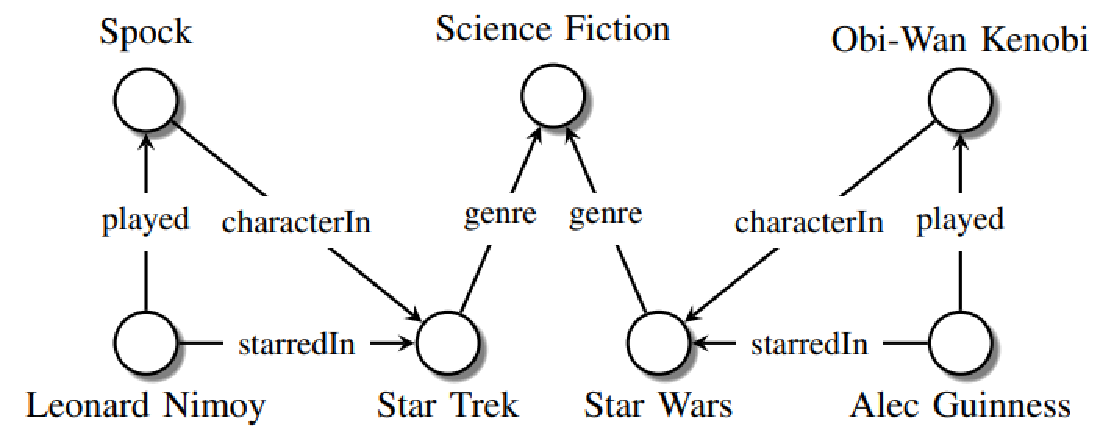
\includegraphics[width=0.67\linewidth]{latex/images/star.pdf}
    % 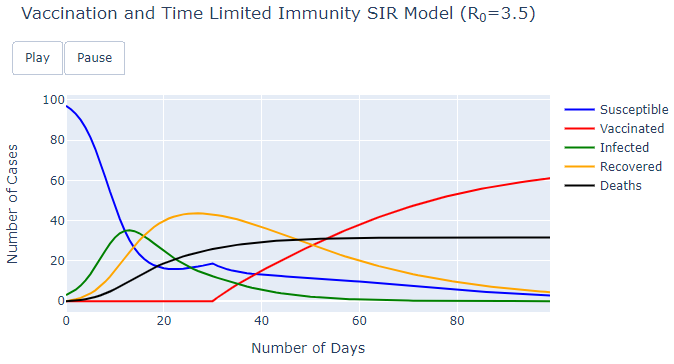
\includegraphics[width=13cm]{latex/images/vacc.PNG}%
    \vspace{-0.2cm}
    \caption{Simple Knowledge Graph. Image reproduced from \cite{leonard}.}
    \label{know}
\end{figure}
\vspace{-0.5cm}

One of the most promising applications of Knowledge Graphs, is to create Machine Learning models able to learn from causality. Knowledge Graph Convolutional Networks (KGCN), represent one of the first successful applications in this ambit \cite{gcn}. Graph Convolutional Networks, are in fact designed to create a vector (embedded) representation of a Knowledge Graph which can then be fed into a Machine Learning model to generate inference paths and provide evidences for the model predictions \cite{net2}. KGCN can be potentially used for either supervised or unsupervised tasks (eg. multi-class classification and clustering).

\section{Bayesian Belief Networks}

Bayesian Belief Networks (BBN), are a type of probabilistic model which makes use of simplifying assumptions so that to reliably define connections between different elements and calculate their probabilities relationships efficiently. By analysing interactions between the different elements, we can finally make use of these type of models in order to discover causal relationships. In a Bayesian Network, nodes represent variables while edges report the probabilistic connections between the different elements. A simple example of a three variables Bayesian Belief Network, is available in Figure \ref{net}.

\begin{figure}[ht!]%
    \centering
    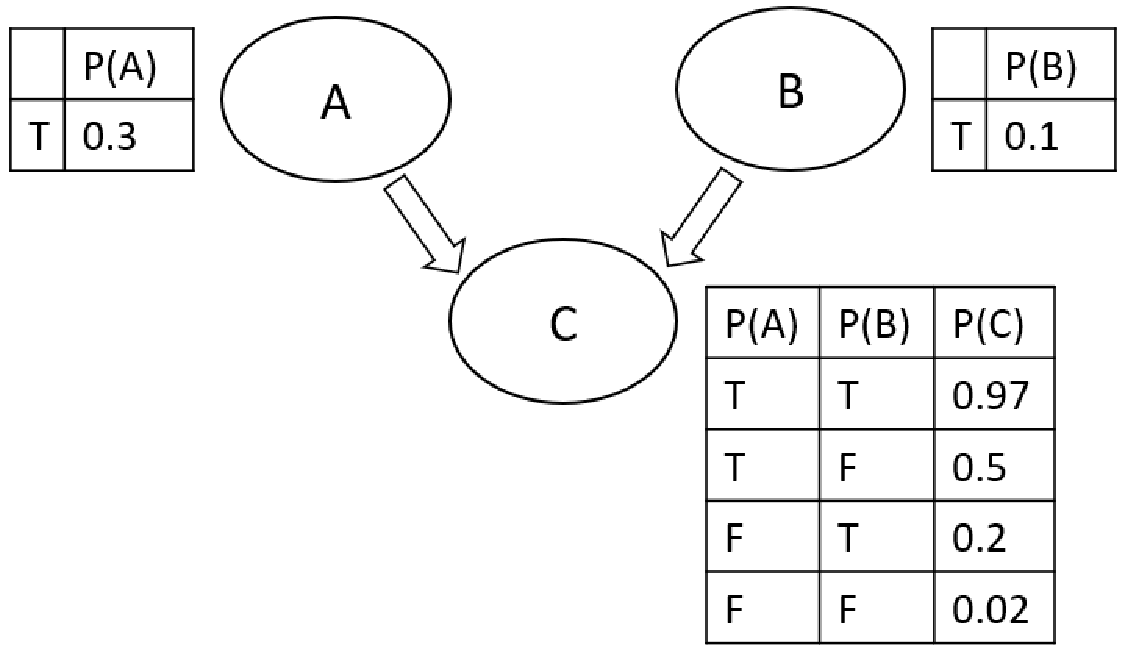
\includegraphics[width=0.7\linewidth]{latex/images/bayes.pdf}
    % 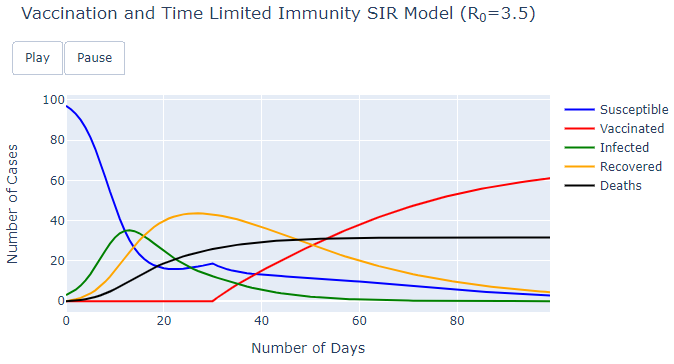
\includegraphics[width=13cm]{latex/images/vacc.PNG}%
    \vspace{-0.2cm}
    \caption{Bayesian Belief Network}
    \label{net}
\end{figure}
\vspace{-0.5cm}

Bayesian Belief Networks, are able to express both conditional dependent and independent variables connections. These type of networks, follow additionally the Markov condition \cite{markov} (provided the parents of every node in a network, each node is conditionally independent of their nondescendent nodes). Finally, using Bayes probabilistic approach (Equation \ref{beq}), we can be able to update the connection probabilities iteratively based on new gathered evidence.

\begin{equation}
P(A|B) = \frac{P(B|A)\times P(A)}{P(B)}
\label{beq}
\end{equation}
\vspace{-0.1cm}
\begin{conditions}
 $A,B$   &  Events \\
 $P(B|A)$ &  Likelihood \\
 $P(A)$   &  Prior \\   
 $P(B)$ & Normalizing Constant \\
 $P(A|B)$ & Posterior
\end{conditions}
\vspace{-0.1cm}

Complex BBNs can be constructed by starting from three basic types of junctions: Chains (e.g. $A \Rightarrow B \Rightarrow C$), Forks (e.g. $A \Leftarrow B \Rightarrow C$) and Colliders (e.g. $A \Rightarrow B \Leftarrow C$). Making use of the three types of junctions and of a technique called d-separation, it can then be possible to reach the Counterfactuals level in the Causality Hierarchy \cite{why}. D-separation, allow us in fact to understand, in Causal Diagrams, if a set of variables is independent of another set when given a third one. 

What distinguishes Bayesian statistic from the classical frequentistic approach, is that we allow to incorporate some level of subjectivity in our model\footnote{Frequentistic probability aims instead for complete objectiveness.} (by combining prior knowledge with evidences). Additionally, in Bayesian statistics, the weight of our prior belief gradually vanishes as more data is provided (therefore converging to the frequentistic approach if given an unlimited amount of data). This case, doesn't instead hold true when talking about causality analysis.

Great research focus by companies such as DeepMind is currently put into using Bayesian Belief Networks as starting point in order to create Causal Bayesian Networks (CBN) \cite{deep}. Causal Bayesian Networks, are nowadays used in order to visually identify and quantitatively measure unfairness patterns in datasets (elements in the data which can lead to Machine Learning models biased towards specific subcategories). Additionally, researches also demonstrated the possibility to use Causal Bayesian Networks in order to identify if not just the data but also the Machine Learning models itself are biased or not towards specific classes \cite{deep2}.

\section{Explainable AI}
One of the major trade-offs in nowadays Machine Learning is model performance against complexity. In fact, complex Deep Learning architectures are usually able to perform better in a wide variety of tasks compared to traditional linear classifiers and regression techniques. This trade-off has been analysed in depth in the 2016 publication "Why should I trust you?" by Ribiero et. al. \cite{xai} and led a new trend in AI to focus on interpretability.

Complex and more accurate models are nowadays referred as \textbf{Black-boxes}. These type of models working progresses are more difficult to comprehend and they are not able to estimate the importance of each feature and how they are related to each other. Some examples of Black Boxes models are neural networks and ensemble models.

On the other hand, simpler and less accurate models such as decision trees and linear regression, are instead regarded as \textbf{White-boxes} and can be much more interpretable. Two of the main measures which can be used in order to estimate the explainability of a model, are the linearity and monotonicity of it's response function \cite{lars}.

\subsection{Model surrogates}

One possible approach which can be used in order to make models more explainable, is to create surrogate versions (approximated versions). This can be done either on a local or global scale.

\begin{itemize}
    \item \textbf{Global Surrogate Model:} in this situation, we create a linear and monotonic approximation of our original non-linear model which is valid for any possible input. In case, the original model was highly non-linear, then creating a Global Surrogate might lead to poor performances.
    \item \textbf{Local Surrogate Model:} are typically implemented when trying to approximate highly non-linear models. Using this type of approach, we can in fact divide our original feature space into different linear subsections. For each of these sections, can then be created a linear model equivalent approximation (e.g. using decision trees and linear models). Local Surrogate Models, are also commonly referred as Local Interpretable Model-Agnostic (LIME).
\end{itemize}

Surrogate models, are trained using the input features and the original model predictions (instead of the ground-truth labels).

In Figure \ref{ex_xai}, is available a simple example showing how a fitted curve might look like, for a regression task, when using either standard black box models or model surrogate techniques. 

\begin{figure}[ht!]%
    \centering
    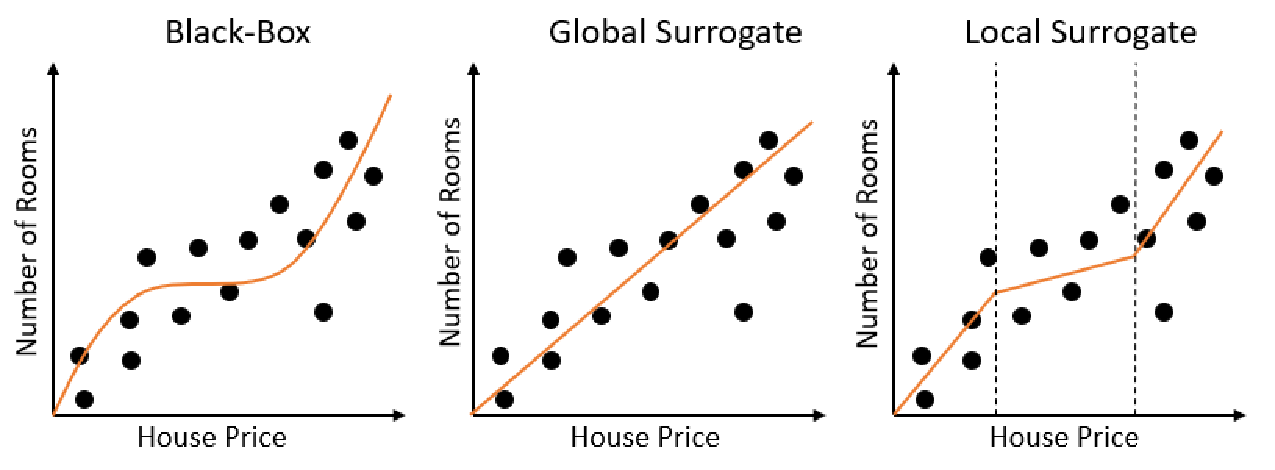
\includegraphics[width=0.75\linewidth]{latex/images/xai_d.pdf}
    % 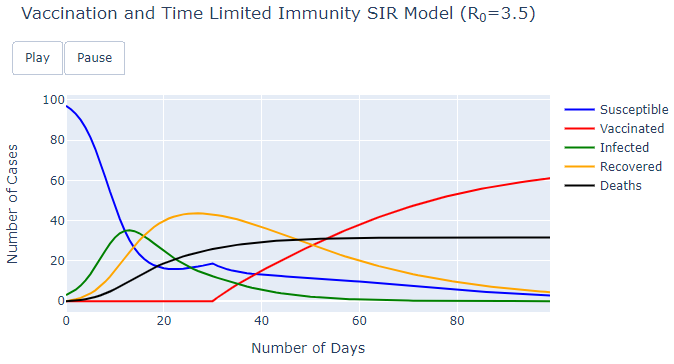
\includegraphics[width=13cm]{latex/images/vacc.PNG}%
    \vspace{-0.2cm}
    \caption{Model Surrogates Example}
    \label{ex_xai}
\end{figure}
\vspace{-0.5cm}

Some alternative approaches which can be used in order to make models more explainable are: Feature Importance, Shapley additive explanations (SHAP), Partial Dependence Plots (PDP) and Gradient/Attention based methods.

\subsection{Bias in AI}

Another key reason why it is important to create Explainable and Causality based Machine Learning models, is to identify and prevent any possible form of bias (e.g. unfair discrimination against any particular class). Bias can potentially arise in fact from either the training dataset itself (e.g. our limited amount of data might not be able to correctly represent the real population distribution) or the model constitution (e.g. our model might unjustifiably prefer one class over the others). Some examples of possible types of bias are: Interaction Bias, Latent Bias and Selection Bias.

\section{Causal Analysis Case Study}


% \section{Faces Responses in Children with ASD}

% % https://www.overleaf.com/learn/latex/algorithms
% \begin{algorithm}[H]
% \SetAlgoLined
% \KwResult{Write here the result }
%  initialization\;
%  \While{While condition}{
%   instructions\;
%   \eIf{condition}{
%   instructions1\;
%   instructions2\;
%   }{
%   instructions3\;
%   }
%  }
%  \caption{How to write algorithms}
% \end{algorithm}

% \begin{algorithm}
% \caption{Calculate $y = x^n$}
% \label{alg1}
% \vspace*{-.4cm}
% \begin{multicols}{2}
% \begin{algorithmic}[1]
%   \REQUIRE $n \geq 0 \vee x \neq 0$
%   \ENSURE $y = x^n$
%   \STATE $y \Leftarrow 1$
%   \IF{$n < 0$}
%   \STATE $X \Leftarrow 1 / x$
%   \STATE $N \Leftarrow -n$
%   \ELSE
%   \STATE $X \Leftarrow x$
%   \STATE $N \Leftarrow n$
%   \ENDIF
%   \WHILE{$N \neq 0$}
%   \IF{$N$ is even}
%   \STATE $X \Leftarrow X \times X$
%   \STATE $N \Leftarrow N / 2$
%   \ELSE[$N$ is odd]
%   \STATE $y \Leftarrow y \times X$
%   \STATE $N \Leftarrow N - 1$
%   \ENDIF
%   \ENDWHILE
% \end{algorithmic}
% \end{multicols}
% \vspace*{-.3cm}
% \end{algorithm}

% The pre-processing part consisted of, firstly loading the data, standardising it and then dividing it in training (70\%) and test sets (30\%) for both the inputs (X) and outputs values (Y). The total number of rows in the data-set was equal to 1906500 (934750 rows about typical children EEG data and 971750 about ASD data). Because of the 70\% against 30\% train/test split ratio, 5338 predictions were made during the training set (1334550/250 time-steps) and 2288 predictions during the test set (571950/250 time-steps).

% I finally decided to train and then test the binary classification results using different algorithms such as: Logistic Regression, Support Vector Machines (SVM), Decision Trees, Linear Discriminant analysis (LDA) and Gaussian Naive Bayes Classifier (GNB). The classification results are show in Table 4.1. At the output, a zero represent a typical child and a one represents a child affected by ASD. The models used attempted to identify if a child is affected or not by ASD using just a single stimulus repetition ($128 channels \times250 timesteps \times1 repetition$).

% {
% \begin{table}[h!]
% \centering
% \begin{tabular}{|c|c|}
% \hline
% Classifier &Accuracy (\%) \\
% \hline
% Logistic Regression & 53  \\
% Support Vector Machines & 53  \\
% Decision Tree & 80  \\
% Linear Discriminant Analysis & 53 \\
% Gaussian Naive Bayes & 60 \\
% \hline
% \end{tabular}
% \caption{ML Classification Accuracy}
% \label{table:1}
% \end{table}
% }

% \begin{lstlisting}[language=Python, caption=LSTM Preprocessing]
% segments = []
% for i in range(0, len(df) - N_TIME_STEPS, step):
%     ch = []
%     for j in range(0, N_FEATURES):
%         ch.append(df.iloc[:, j].values[i: i + N_TIME_STEPS])
%     segments.append(ch)
% labels = []
% for i in range(0, len(df) - N_TIME_STEPS, step):
%     label = stats.mode(df['Label'][i: i + N_TIME_STEPS])[0][0]
%     labels.append(label)
% labelsl = np.asarray(pd.get_dummies(labels), dtype = np.float32)
% reshaped_segments = np.asarray(segments, dtype= np.float32).reshape(-1, N_TIME_STEPS, N_FEATURES)
% X_train, X_test, y_train, y_test = train_test_split(
%         reshaped_segments, labelsl, test_size=0.2, random_state=RANDOM_SEED)
% \end{lstlisting}

% {
% \begin{table}[h!]
% \centering
% \begin{tabular}{|c|c|}
% \hline
% Parameter &Number \\
% \hline
% Time Steps & 250  \\
% Features & 128  \\
% Steps & 25  \\
% Classes & 2 \\
% Hidden Units & 32 \\
% L2 Regularization & 0.0015 \\
% Learning Rate & 0.0025 \\
% Epochs & 50 \\
% Batch Size & 256 \\
% \hline
% \end{tabular}
% \caption{LSTM Parameters}
% \label{table:1}
% \end{table}
% }



% {
% \begin{table}[h!]
% \centering
% \begin{tabular}{l|l|c|c|c}
% \multicolumn{2}{c}{}&\multicolumn{2}{c}{}&\\
% \cline{3-4}
% \multicolumn{2}{c|}{}&Negative (0)&Positive (1)&\multicolumn{1}{c}{Total}\\
% \cline{2-4}
% \multirow{}{}{}& Negative (0) & $1093$ & $29$ & $1122$\\
% \cline{2-4}
% & Positive (1) & $22$ & $1144$ & $1166$\\
% \cline{2-4}
% \multicolumn{1}{c}{} & \multicolumn{1}{c}{Total} & \multicolumn{1}{c}{$1115$} & \multicolumn{    1}{c}{$1173$} & \multicolumn{1}{c}{$2288$}\\
% \end{tabular}
% \caption{LSTM Confusion Matrix}
% \label{table:1}
% \end{table}
% }

% The model consisted of: 
% \begin{enumerate}
% \itemsep0em
% \item One 2D Convolutional Layer of 64 filters, a kernel size of $5\times5$, a ReLU (Rectified Linear Unit, Equation 4.3) function and same padding. 
% \useshortskip
% \begin{align}
% \ f(x) = max(0,x)
% \label{eq:3}
% \end{align}
% \useshortskip
% \item Another 2D Convolutional Layer having 32 filters, a kernel size of $5\times5$, a ReLU (rectified linear unit) function, same padding and an L2 regularisation coefficient of 0.01 (to prevent overfitting). 
% \item A 2D MaxPooling layer of $2\times2$ size.
% \item A Dropout layer of 0.2 intensity (in order to avoid over-fitting the data).
% \item A layer to first flatten the data from three dimensions to just one, and then another one to condense the input to give to the classifier 128 features (always using the ReLU function and L2 regularisation).
% \item A second Dropout layer of 0.5 intensity.
% \item Finally, a Dense layer (of two neurons) to produce the classification result, using a Softmax activation function. The Softmax function (Equation 4.4) will take in this case the two inputs from the neurons and convert them in two probabilities that sums up to one. The greater probability was rounded up/down to either one or zero to represent the CNN output choice (Typical(0), ASD(1)).
% % \setlength{\floatsep}{-2pt}
% \begin{align}
% \ \sigma(x)_{j} = \frac{e^{x_{j}}}{\sum_{k=1}^{k} e^{x_{k}}} && \text{for j=1,\dots,k}
% \label{eq:3}
% \end{align}
% % \useshortskip
% \end{enumerate}

% In order to optimise the training, the Adam (Adaptive Moment Estimation) gradient descent algorithm was used, and the cross-entropy function was used to compute the model loss. The cross-entropy function ($H_{y'}(y)$), in a binary classification case can be calculated by using Equation 4.5.
% \useshortskip
% \begin{align}
% \ H_{y'}(y) = \sum_{i} (y_{i}'\log(y_{i}) + (1 - y_{i}')\log(1 - y_{i}))
% \label{eq:3}
% \end{align}
% \useshortskip
% \begin{conditions}
%  y_{i}'  &  expected model output \\
%  y_{i}     &  real model output \\
% \end{conditions}
% \useshortskip
% This model achieved an overall validation accuracy of 94.58\% in just thirty epochs of training. 


% {
% \begin{table}[h!]
% \centering
% \begin{tabular}{l|l|c|c|c}
% \multicolumn{2}{c}{}&\multicolumn{2}{c}{}&\\
% \cline{3-4}
% \multicolumn{2}{c|}{}&Negative (0)&Positive (1)&\multicolumn{1}{c}{Total}\\
% \cline{2-4}
% \multirow{}{}{}& Negative (0) & $1001$ & $100$ & $1101$\\
% \cline{2-4}
% & Positive (1) & $24$ & $1163$ & $1187$\\
% \cline{2-4}
% \multicolumn{1}{c}{} & \multicolumn{1}{c}{Total} & \multicolumn{1}{c}{$1025$} & \multicolumn{    1}{c}{$1263$} & \multicolumn{1}{c}{$2288$}\\
% \end{tabular}
% \caption{CNN Confusion Matrix}
% \label{table:1}
% \end{table}
% }